\documentclass{article}
\usepackage{graphicx}
\usepackage{mhchem}
\usepackage{tikz}
\usepackage{pgfplots}
\usepackage{pgfplotstable}
\usepackage{filecontents}
\usepackage[T1]{fontenc}
\usepackage[utf8]{inputenc}
\usepackage[english, russian]{babel}

\graphicspath{ {./data/} } 

\title{Исследование явления осмоса на базе лабораторного стенда и расчёт зависимостей}
\author{Нестеров И.Д.}
\date{}

\begin{document}
    \selectlanguage{russian}
    \maketitle
    \tableofcontents
    \newpage

    \addcontentsline{toc}{section}{Введение}
    \section*{Введение}

        \hspace*{4mm}\textbf{\textit{Цель работы:}} Ознакомиться и научиться проводить исследования осмотических
        процессов в частности провести расчёты осмотического давления и осмотического потока, используя законы Фика.
        
        \addcontentsline{toc}{subsection}{Осмос}
        \subsection*{Осмос}
            \hspace*{4mm}\textit{Осмос} – частный случай \textit{диффузии}. Другими словами, это диффузия воды
            через полупроницаемую мембрану вниз по градиенту концентрации, когда
            растворенное вещество не может диффундировать через мембрану, а вода может,
            если мембрана проницаема для воды, но не для растворенного
            вещества. Вода будет выравнивать свою собственную концентрацию путем
            диффундирования в сторону с более низкой концентрацией воды.

            \begin{itemize}
                \item Вода считается универсальным растворителем -
                она связывает и растворяет полярные или заряженные
                молекулы (растворённые вещества)

                \item Поскольку растворённые вещества не могут
                проникнуть через клеточную мембрану без посторонней
                помощи, вода будет перемещаться, чтобы уравнять оба
                раствора

                \item При более высокой концентрации растворённого
                вещества в растворе меньше свободных молекул воды,
                поскольку вода связана с растворённым веществом
            \end{itemize}

            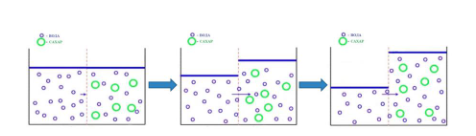
\includegraphics[width=0.9\textwidth]{Osmos.png}
        
        \newpage
        \addcontentsline{toc}{subsection}{Осмотическое давление}
        \subsection*{Осмотическое давление}
            \hspace*{4mm}\textit{Осмотическое давление} можно определить как минимальное давление, которое необходимо
            приложить к раствору, чтобы остановить поток молекул растворителя через
            полупроницаемую мембрану (осмос). Это коллигативное свойство, которое
            зависит от концентрации частиц растворенного вещества в растворе.
            Для вычисления осмотического давления можно воспользоваться уравнением Вант-Гоффа:

            \begin{equation}
                \pi = iCRT    
            \end{equation}
            
            где $\pi$ – осмотическое давление,
            $i$ - изотонический коэффициент,
            $C$ - концентрация растворённого вещества,
            $R$ – универсальная газовая постоянная,
            $T$ – температура вещества. \\

            Для воды $i = 1.015$

        \addcontentsline{toc}{subsection}{Осмотический поток}
        \subsection*{Осмотический поток}
            \hspace*{4mm}Для расчёта потока используем стандартную формулу для диффузного потока, однако с учетом того, что осмос
            является односторонним процессом диффузии, где движущая жидкость является
            вода, интерпретируя закон Фика под эту цель.

            \begin{center}
                Первый закон Фика:

                \begin{equation}
                    J = -D\frac{dC}{dx}    
                \end{equation}
            \end{center}
            
            где $D$ - коэффициент диффузии, $\frac{dC}{dx}$ - градиент концентрации
            вещества. \\

    \newpage
    \addcontentsline{toc}{section}{Ход работы}
    \section*{Ход работы}

        \addcontentsline{toc}{subsection}{Растворы}
        \subsection*{Растворы}
            \hspace*{4mm}Было приготовлено два раствора \ce{CuSO4*5H2O} с разными концентрациями.
            Концентрация первого раствора составляла 10\%, второго - 20\%.


        \addcontentsline{toc}{subsection}{Установка}
        \subsection*{Установка}
            \hspace*{4mm}Для наблюдения и демонстрации осмотических процессов идеально
            подходит камера для осмоса и электрохимии. В обычной форме
            устройство имеет две стеклянные концевые камеры и двух резиновых
            уплотнительных колец, соединенных с помощью фланцевого держателя. Все
            камеры располагают стеклянную короткую трубку с резьбой GL25, на которую
            можно накрутить винтообразную крышку с кольцом уплотнения (25/8 мм).
            Экспериментируя с осмосом, стеклянные капиллярные трубки вставляют в эти
            соединительные крышки. \\
        
            \includegraphics*[width=0.8\textwidth]{tools1.png} \\

            \hspace*{4mm}Чтобы собрать двухкамерное устройство,
            Необходимо расположить подходящую полупроницаемую мембрану,
            изготовленную из целлофана, между двумя уплотнительными кольцами, а затем
            скрепить вместе две камеры прямоугольный зажимом, вместе с
            уплотнительными кольцами. \\

            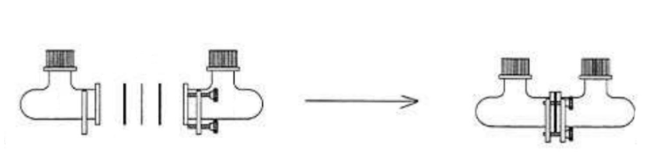
\includegraphics[scale=0.65]{tools2.png} \\

            \begin{center}
                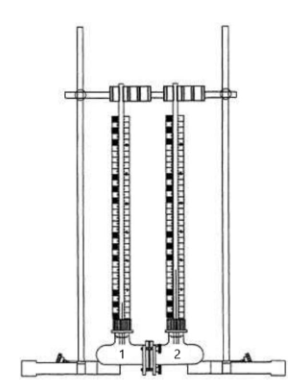
\includegraphics[scale=0.8]{tools3.png}
                \vspace*{4mm}
            \end{center}

            Характеристики компонентов:

            \begin{itemize}
                \item Внешний диаметр камеры: $D_o = 3.4$ см
                \item Внутренний диаметр камеры: $D_i \approx 3$ см
                \item Диаметр фланца: $D_o = 4.7$ см
                \item Толщина фланца: $d_o = 1$ мм
                \item Длина сегмента: $L \approx 90$ мм
                \item Высота: $H \approx 85$ мм
                \item Объём одного сегмента: $V \approx 65$ мл
            \end{itemize}
            \newpage

        \addcontentsline{toc}{subsection}{Наблюдения}
        \subsection*{Наблюдения}
            \hspace*{4mm}После сбора установки и начала эксперимента каждые 5 минут производились измерения высоты
            столбцов с растворами. \\

            Динамика высоты жидкости в первом сосуде, в котором концентрация составляла 10\%:
            \vspace*{8mm}

            \begin{tikzpicture}
                \begin{axis}[scale only axis,
                        ylabel = {$h$, см},
                        xlabel = {$t$, с},
                        xmax=35,
                        ymin=15, ymax=17,
                        xtick={0,5,...,30},
                        ytick={15.2,15.6,...,16.6},
                        axis lines=middle,
                        grid=both   
                    ] 
                    \addplot[only marks] table [col sep=comma] {./data/experiment1.csv};
                \end{axis}
            \end{tikzpicture}
            \newpage

            Динамика высоты жидкости во втором сосуде, в котором концентрация составляла 20\%:
            \vspace*{8mm}

            \begin{tikzpicture}
                \begin{axis}[scale only axis,
                        ylabel = {$h$, см},
                        xlabel = {$t$, с},
                        xmax=35,
                        ymin=17, ymax=21,
                        xtick={0,5,...,30},
                        ytick={17.5,18.0,...,20.5},
                        axis lines=middle,
                        grid=both   
                    ] 
                    \addplot[only marks] table [col sep=comma] {./data/experiment2.csv};
                \end{axis}
            \end{tikzpicture}
            \newpage

    \addcontentsline{toc}{section}{Обработка данных}    
    \section*{Обработка данных}
        \addcontentsline{toc}{subsection}{Вычисление осмотического давления и его временной зависимости}
        \subsection*{Вычисление осмотического давления и его временной зависимости}

            \hspace*{4mm}В соответствии с формулой (1) могут быть вычислены значения осмотического давления в сосудах: \\

            \begin{equation}
                \pi = i\frac{m}{M}\frac{RT}{V_{0} \pm \Delta{V}}
            \end{equation}

            Где $\Delta{V}$ - объём жидкости, которая перетекла из сосуда в сосуд. \\
            \\
            Зависимость осмотического давления от времени отражена на графиках ниже.\\
            
            Для первого сосуда:
            \vspace*{4mm}

            \begin{tikzpicture}
                \begin{axis}[scale only axis,
                        xlabel = {$t$, с},
                        ylabel = {$P$, кПа},
                        xmax=35,
                        ymin=1518.10, ymax=1518.60,
                        xtick={0,5,...,30},
                        ytick={1518.00,1518.05,...,1518.55},
                        axis lines=middle,
                        grid=both
                    ]
                    \addplot[only marks] table [col sep=comma] {./data/pressure1.csv};
                    \addplot[smooth, color=gray] coordinates {(0,1518.2)(30,1518.4919)};
                    \addlegendentry{$P(t) = 9.73\cdot10^{-3}t+1518.2$}
                \end{axis}
            \end{tikzpicture}
            \newpage
            Для второго сосуда:
            \vspace*{4mm}

            \begin{tikzpicture}
                \begin{axis}[scale only axis,
                        xlabel = {$t$, с},
                        ylabel = {$P$, кПа},
                        xmax=35,
                        ymin=3033.92, ymax=3037.00,
                        xtick={0,5,...,30},
                        ytick={3033.90,3034.30,...,3036.47},
                        axis lines=middle,
                        grid=both
                    ]
                    \addplot[only marks] table [col sep=comma] {./data/pressure2.csv};
                    \addplot[smooth, color=gray] coordinates {(0,3036.65)(30,3034.121)};
                    \addlegendentry{$P(t) = -8.43\cdot10^{-2}t+3036.65$}
                \end{axis}
            \end{tikzpicture}
        
        \newpage
        \addcontentsline{toc}{subsection}{Вычисление осмотического потока}
        \subsection*{Вычисление осмотического потока}

        В соответствии с формулой (2) величина осмотического потока может быть приблизительно вычислена следующим образом:

        \begin{equation}
            J = -D\frac{|\Delta{C}|}{\Delta{x}} = -D\frac{|C_{1} - C_{2}|}{\Delta{x}}
        \end{equation}

        \vspace*{4mm}
        Значение коэффициента диффузии для воды: $D \approx 10^{-9}$

        Была установлена зависимость осмотического потока с течением времени:
        \vspace*{4mm}

        \begin{tikzpicture}
            \begin{axis}[scale only axis,
                    xlabel = {$t$, с},
                    ylabel = {$|J|$, моль/м$м^2$с},
                    xmax=35,
                    ymin=997.5, ymax=1000.2,
                    xtick={0,5,...,30},
                    ytick={998.0,998.5,...,1000.0},
                    axis lines=middle,
                    grid=both
                ]
                \addplot[only marks] table [col sep=comma] {./flow.csv};
                \addplot[smooth, color=gray] coordinates {(0,1000)(33,997.954)};
                \addlegendentry{$|J(t)| = -6.2\cdot10^{-2}t+1000$}
            \end{axis}
        \end{tikzpicture}

    \newpage
    \addcontentsline{toc}{section}{Результаты и Выводы}
    \section*{Результаты и Выводы}

    \hspace*{4mm}В результате проведённых опытов по изучению осмотических процессов с медным купоросом
    были вычислены экспериментально осмотические давления для обоих сосудов, а также осмотический поток
    через полупроницаемую мембрану.

\end{document}